% Nikolai Nielsens "Fysiske Fag" preamble
\documentclass[a4paper,11pt]{article}
\usepackage[english]{babel}
\usepackage{Nikolai}
\usepackage[dvipsnames]{xcolor}
\usepackage[margin=0.75in]{geometry}
\usepackage{wrapfig}

\usepackage{pdfpages}

\usepackage{listings}
\usepackage{color}
\definecolor{Maroon}{RGB}{175,50,53}
\definecolor{OliveGreen}{RGB}{60,128,49}
\definecolor{Orange}{RGB}{245,129,55}

\lstset{ %
	language=python,
	numbers=left,
	stepnumber=1,
	breaklines=true,
	keepspaces=true,
	showstringspaces=false, 
	tabsize=4,
	basicstyle=\footnotesize\ttfamily,
	keywordstyle=\bfseries\color{Maroon},
	commentstyle=\itshape\color{OliveGreen},
	identifierstyle=\color{blue},
	stringstyle=\color{Orange},
}

% Til nummerering af ligninger. Så der står (afsnit.ligning) og ikke bare (ligning)
\numberwithin{equation}{section}

\newcommand{\coef}[1]{_{[#1]}}

% Header
%\usepackage{fancyhdr}
%\head{}
%\pagestyle{fancy}

%Titel
\title{Visualisation of concepts in condensed matter physics}
\author{Nikolai Plambech Nielsen, LPK331}
\date{2018-06-13}

\begin{document}
	
	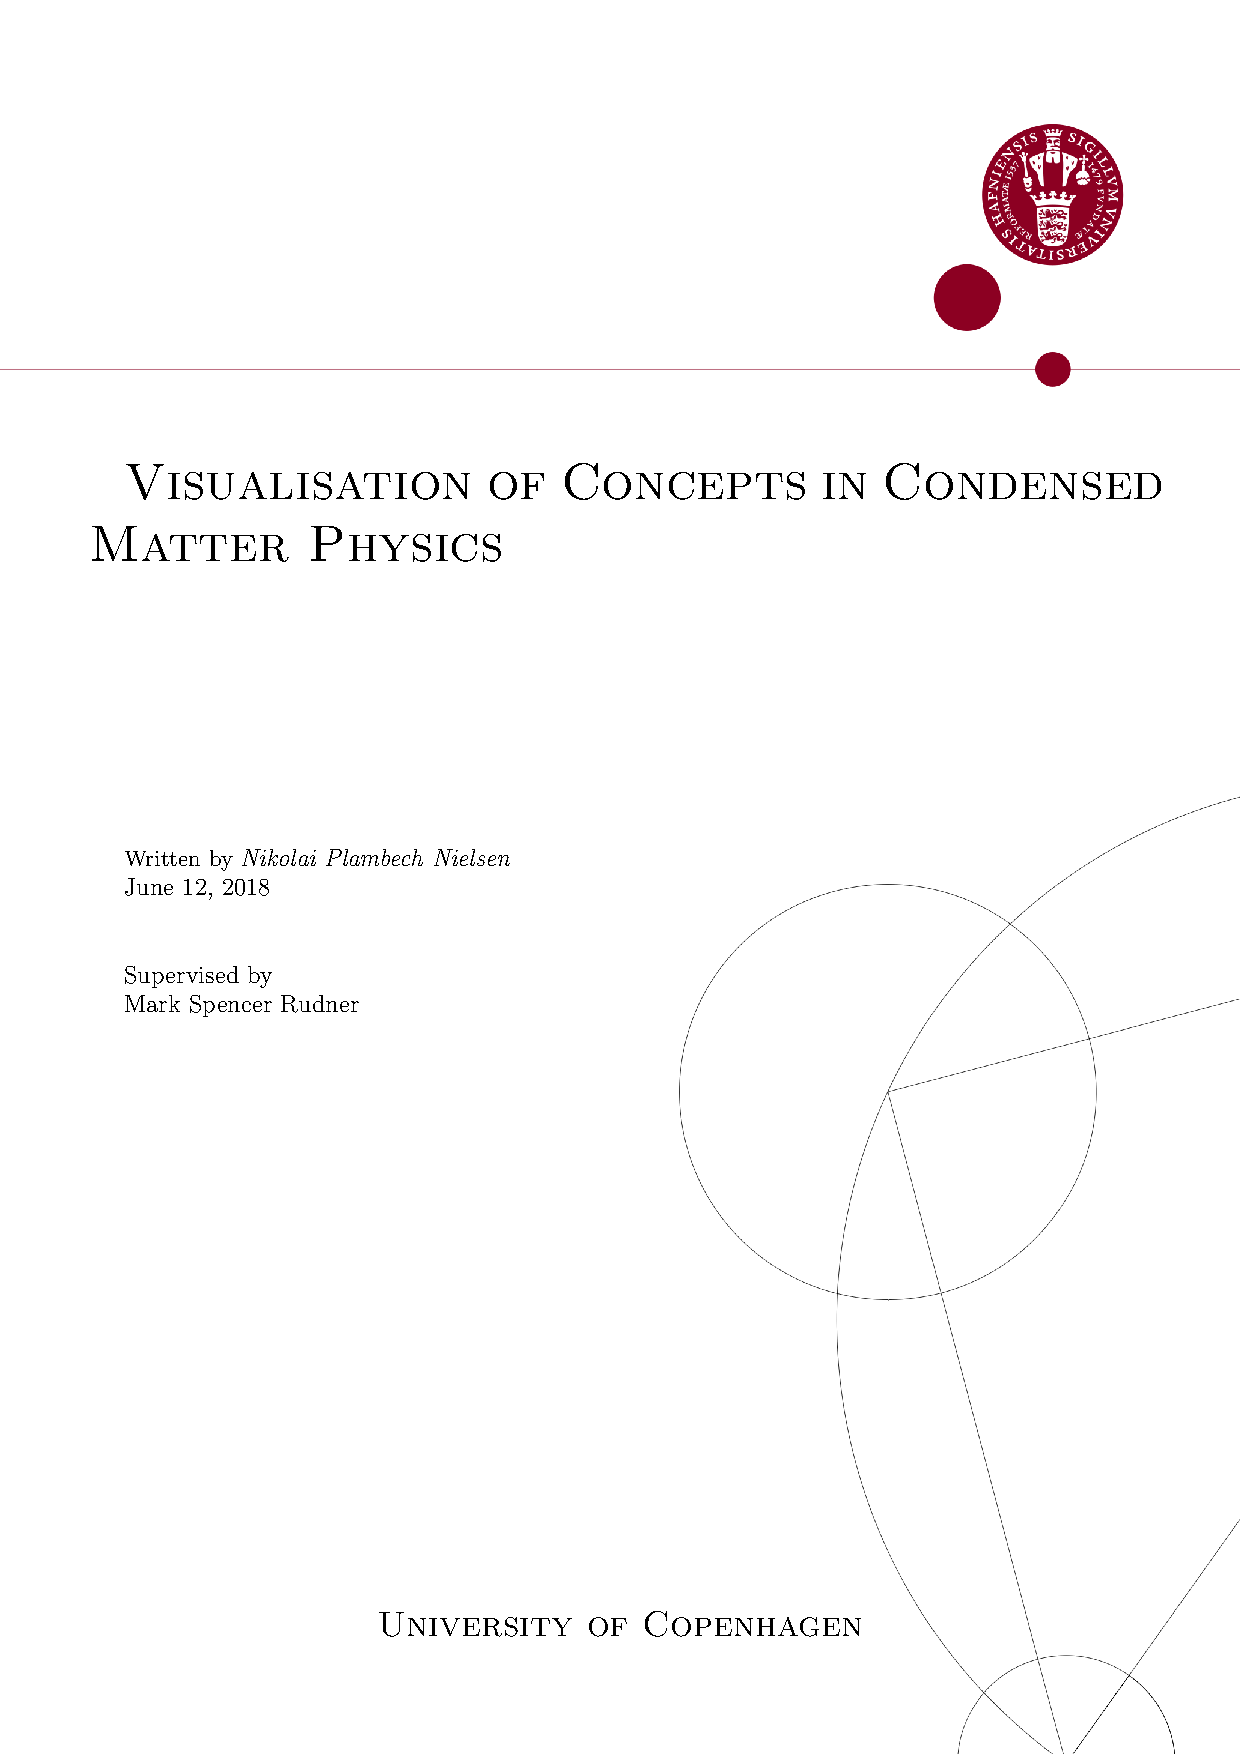
\includepdf[pages=-]{figures/frontpage.pdf}
	
	\pagenumbering{roman}
	
	\begin{abstract}
		In this thesis we explore key concepts in the field of condensed matter physics and translate these into visualisations using the computer programming language Python. Concepts explored include the geometry of crystal structures, families of lattice planes, neutron scattering and the band structure of two dimensional materials. Four distinct programs are written to visualize each of these concepts, and they are bundled into one open-source software package available at \url{https://github.com/NikolaiNielsen/Bachelor}, along with documentation on its use.
	\end{abstract}
	\section*{Acknowledgements}
	This thesis was brought about with the tremendous help from my supervisor, Mark Spencer Rudner. I am grateful for your patience and guidance in helping me write this thesis. It would certainly not have been nearly as easy or with the same quality without you.
	
	
	\tableofcontents
	
	\newpage
	
	\pagenumbering{arabic}
	\setcounter{page}{1}
	\subfile{introduction.tex}
	
	\subfile{lattices.tex}
	
	\subfile{reciprocal.tex}
	
	\subfile{2D_band_structure.tex}
	
	\subfile{discussion.tex}
	
	\bibliography{ref}
	\bibliographystyle{ieeetr}
	
	\newpage
	\appendix
	\subfile{latticeClassification.tex}
	
\end{document}